\documentclass[11pt]{article}
 \pdfminorversion=4
\usepackage[utf8]{inputenc}
\usepackage{amsfonts,epsfig}
\usepackage[hyphens]{url}
%\usepackage{hyperref}
%\usepackage{breakurl}
\usepackage{comment}

\usepackage{natbib}

\linespread{1.25}

\usepackage{relsize}
\usepackage{fancyvrb}
\usepackage{amsmath, amssymb}
%%% Document layout, margins
\usepackage{geometry}
\geometry{letterpaper, textwidth=6.5in, textheight=9in, marginparsep=1em}
%%% Section headings
\usepackage{sectsty}
\usepackage{caption}
\usepackage{subcaption}
\usepackage[normalem]{ulem}
\sectionfont{\sffamily\bfseries\upshape\large}
\subsectionfont{\sffamily\bfseries\upshape\normalsize}
\subsubsectionfont{\sffamily\mdseries\upshape\normalsize}
\makeatletter
\renewcommand\@seccntformat[1]{\csname the#1\endcsname.\quad}

\makeatletter
\def\@maketitle{%
  \begin{center}%
  \let \footnote \thanks
    {\large \@title \par}%
    {\normalsize
      \begin{tabular}[t]{c}%
        \@author
      \end{tabular}\par}%
    {\small \@date}%
  \end{center}%
}
\makeatother


\title{\bf Bayesian leave-one-out cross-validation for non-factorizable normal models\footnote{
We thank Daniel Simpson for useful discussion and the Academy of Finland
(grants 298742, 313122) for partial support of this work.
}\vspace{.1in}}
\author{Paul-Christian B\"{u}rkner\footnote{Department of Psychology, University of M\"{u}nster, Germany.}
  \and Jonah Gabry\footnote{Applied Statistics Center and Institute for Social and Economic Research and Policy, Columbia University, USA.}
  \and Aki Vehtari\footnote{Department of Computer Science, Aalto University, Finland.
}\vspace{.1in}}
\date{\today \vspace{-.1in}}
\begin{document}\sloppy
\maketitle
\thispagestyle{empty}

\begin{abstract}
Cross-validation can be used to measure a model's predictive accuracy for the
purpose of model comparison, averaging, or selection. Standard leave-one-out
cross-validation  (LOO-CV) requires the likelihood to be factorizable, but many
important models in temporal  and spatial statistics do not have this property.
We derive how to compute and validate both exact and approximate LOO-CV for
Bayesian non-factorizable models with a multivariate normal likelihood.
In a case study, we apply this method to lagged simultaneously autoregressive 
(SAR) models.

\textbf{Keywords:} cross-validation, Pareto-smoothed importance-sampling,
  non-factorizable models, SAR models.
\end{abstract}


\section{Introduction}

%After fitting a statistical model we often want to assess its predictive
%accuracy 
In the absence of new data, cross-validation is a general approach for evaluating
a statistical model's predictive accuracy for the purpose of model comparison, 
averaging, or selection \citep{geisser1979, hoeting1999, ando2010, vehtari2012}.
One widely used variant of
cross-validation is \emph{leave-one-out cross-validation} (LOO-CV), where
observations are left out one at a time and then predicted based on the model
fit to the remaining data. Predictive accuracy is evaluated by first computing
the expected log predictive density of the left-out observation and then taking
the sum of these values over all observations to obtain the expected log
predictive density (ELPD) as a single measure of predictive accuracy.
Exact LOO-CV is costly, as it requires fitting the model as many
times as there are observations in the data. Depending on the size of the data,
complexity of the model, and estimation method, this can be practically
infeasible as it simply requires too much computation time. 
For this reason, approximate versions of LOO-CV have been developed 
\citep{gelfand1992, vehtari2017loo}, most recently using 
Pareto-smoothed importance-sampling \citep[PSIS; ][]{vehtari2017loo, vehtari2017psis}.

A standard assumption of any such LOO-CV approach is that the joint likelihood
of the model over all observations has to be factorizable. That is, the
observations have to be pairwise conditionally independent given the model
parameters. However, many important models do not have this property.
Particularly in temporal and spatial statistics it is common to
fit models with multivariate normal likelihoods that have structured covariance
matrices such that the likelihood does not factorize. This is typically due to the 
fact that observations depend on other observations from different time periods 
or different spatial units in addition to the dependence on the model parameters. 

In this short paper we show how equations derived in \cite{sundararajan2001} can
be repurposed and combined with PSIS to allow for performing efficient
approximate LOO-CV for \emph{any} multivariate normal Bayesian model with an
invertible covariance matrix, regardless of whether or not the likelihood
factorizes. We also provide equations for computing exact LOO-CV for these
models, which can be used to validate the approximation. Throughout, a Bayesian
model specification and estimation via Markov chain Monte Carlo (MCMC) is
assumed. In an online supplementary material we provide R code demonstrating how to
carry out the approximation described in the paper.\footnote{
Supplemental materials available at  \url{https://mc-stan.org/loo/articles/loo2-non-factorizable.html}.}

Although our proposed method makes use of standard multivariate normal theory, 
we think there is value in explicitly presenting this theory to applied researchers,  
along with a recommended workflow for implementation in practice.


\section{Pointwise log-likelihood for non-factorizable normal models}
\label{sec-pointwise}

When computing \emph{exact} LOO-CV for a Bayesian model we need to compute the
log leave-one-out predictive densities $\log{p(y_i | y_{-i})}$ for every
response value $y_i, \: i = 1, \ldots, N$, where $y_{-i}$ denotes all response
values except observation $i$. This requires fitting the model $N$ times. For
\emph{approximate} LOO-CV using only a single model fit, we instead calculate
the pointwise log-likelihood (the log-predictive density evaluated at
each data point), without leaving out any observations, and then apply an
importance sampling correction \citep{gelfand1992, vehtari2017loo}.

The pointwise log-likelihood is straightforward to compute for
\emph{factorizable} models in which response values are conditionally
independent given the model parameters $\theta$ and the likelihood can be
written in the familiar form
%
\begin{equation}
p(y \,|\, \theta) = \prod_{i=1}^N p(y_i \,|\, \theta).
\end{equation}
%
When $p(y)$ can be factorized in this way, the conditional pointwise
log-likelihood can be obtained easily by computing $\log p(y_i \,|\, \theta)$
for each $i$.

The situation is more complicated for \emph{non-factorizable} models in which
response values are not conditionally independent. When there is residual
dependence even after accounting for the model parameters, the conditional
pointwise log-likelihood has the general form $\log p(y_i \,|\, y_{-i},
\theta)$. Computing this pointwise log-likelihood for non-factorizable models is 
often impossible, but there is a large class of multivariate normal models for which 
an analytical solution is available.

\cite{sundararajan2001} provide equations for the predictive mean and standard
deviation for a zero-mean Gaussian process model with prior covariance $K$ and
residual standard deviation $\sigma$,
%
\begin{equation}
\label{gp}
y \sim {\mathrm N}(0, \, K+\sigma^2 I),
\end{equation}
%
where $I$ is the identity matrix of appropriate dimension and $C = K+\sigma^2 I$
is the covariance matrix of the model. In the context of Gaussian process models, 
these equations did not actually find much practical application because, in most
cases, Gaussian processes are combined with a factorizable likelihood so that
simpler equations for univariate distributions can be applied. But the
derivations of Sundararajan and Keerthi's equations make no use of the special
form of $C$ for Gaussian process models and thus immediately generalize to the
case of an arbitrary invertible covariance matrix $C$.

For such models, the LOO predictive mean and standard deviation can be computed
using the equations from \cite{sundararajan2001} as follows:
%
\begin{align}
\label{ypredpars}
  \mu_{\tilde{y},-i} &= y_i-\bar{c}_{ii}^{-1} g_i \nonumber \\
  \sigma_{\tilde{y},-i} &= \sqrt{\bar{c}_{ii}^{-1}},
\end{align}
%
where $g_i = \left[C^{-1} y\right]_i$ and
$\bar{c}_{ii} = \left[C^{-1}\right]_{ii}$.
The log predictive density of the $i$th observation is
%
\begin{equation}
  \log p(y_i \,|\, y_{-i},\theta)
  = - \frac{1}{2}\log(2\pi)
  - \frac{1}{2}\log \sigma^2_{-i}
  - \frac{1}{2}\frac{(y_i-\mu_{-i})^2}{\sigma^2_{-i}},
\end{equation}
%
and expressing this same equation in terms of $g_i$ and $\bar{c}_{ii}$, we
obtain\footnote{ Note that \cite{vehtari2016} has a typo in the corresponding
Equation 34.}:
%
\begin{equation}
\label{logpointwise}
  \log p(y_i \,|\, y_{-i},\theta)
  = - \frac{1}{2}\log(2\pi)
  + \frac{1}{2}\log \bar{c}_{ii}
  - \frac{1}{2}\frac{g_i^2}{\bar{c}_{ii}}.
\end{equation}
%
The above equations may also be derived directly from multivariate normal theory. 
Evaluating equation \eqref{logpointwise} for each $y_i$ provides the pointwise
log-likelihood values required for the PSIS-LOO-CV approximation. 
While the computational cost in the factorizable case is only $O(n)$, 
it is much higher in the non-factorizable case. The latter is usually dominated by the 
computation of $C^{-1}$, which is in $O(n^3)$ for dense $C$. However, if $C$ is 
sparse (see below for an example) or reduced rank, the computational will be less than $O(n^3)$.

It often requires additional work to take a given multivariate normal
model and express it in the same form as the zero mean Gaussian process 
in \eqref{gp} in order to apply the equations for the predictive 
mean and standard deviation. Consider, for example, the lagged simultaneously 
autoregressive (SAR), which has many applications in both the social sciences 
(e.g., economics) and natural sciences (e.g., ecology). The model is given by 
%
\begin{equation}
y = \rho W y + \eta + \epsilon,
\end{equation}
%
or equivalently 
%
\begin{equation}
(I - \rho W) y = \eta + \epsilon,
\end{equation}
%
where $\rho$ is a scalar spatial correlation parameter and $W$ is a user-defined matrix of weights. 
The matrix $W$ has entires $w_{ii} = 0$ along the diagonal and the off-diagonal entries $w_{ij}$
are larger when units $i$ and $j$ are closer to each other but mostly zero as well. In a linear model, 
the predictor term is $\eta = X \beta$, with design matrix $X$ and regression coefficients $\beta$,
but the definition of the lagged SAR model holds for arbitrary $\eta$, so 
these results are not restricted to the linear case.  

If we have $\epsilon \sim \mathrm{N}(0, \sigma^2 I)$, it follows that 
%
\begin{equation}
\label{lagsar}
(I - \rho W) y \sim \mathrm{N}(\eta, \sigma^2 I),
\end{equation}
%
but this standard way of expressing the model is not compatible with the equations 
from \cite{sundararajan2001}. To make the lagged SAR model reconcilable with 
these equations we need to rewrite it as follows (conditional on 
$\rho$, $\eta$, and $\sigma$):
%
\begin{equation}
y - (I - \rho W)^{-1} \eta \sim \mathrm{N}\left(0, \sigma^2 (I - \rho W)^{-1} (I - \rho W)^{-T} \right),
\end{equation}
%
or more compactly, with $\widetilde{W} = (I - \rho W)$, 
%
\begin{equation}
y - \widetilde{W}^{-1} \eta \sim \mathrm{N}\left(0, \sigma^2  (\widetilde{W}^T \widetilde{W})^{-1} \right).
\end{equation}
%
Written in this way, the lagged SAR model has the same form as the zero mean Gaussian process from 
\eqref{gp}. Accordingly, we can compute the leave-one-out predictive densities with the equations from 
\cite{sundararajan2001}, replacing $y$ with $y - \widetilde{W}^{-1} \eta$ and taking the covariance
matrix $C$ to be $\sigma^2  (\widetilde{W}^T \widetilde{W})^{-1}$. 
This implies $C^{-1}=\sigma^{-2}\widetilde{W} \widetilde{W}^T$ and so the overall computational cost is 
dominated by $\widetilde{W}^{-1} \eta$. In SAR models, $W$ is usally sparse and so is $\widetilde{W}$. 
Thus, if sparse matrix operations are used, then the computational cost for $C^{-1}$ will be less than 
$O(n^2)$ and for $\widetilde{W}^{-1}$ it will be less than $O(n^3)$ (depending on number of non-zeros and the fill pattern).

\section{Approximate LOO-CV for non-factorizable normal models}
\label{sec-approx}

The conditional pointwise log-likelihood is the only required input to the
PSIS-LOO-CV algorithm from \cite{vehtari2017loo} and thus Sundararajan and
Keerthi's repurposed equations allow for approximate LOO-CV for \emph{any} model
that can be expressed conditionally in terms of a multivariate normal with
invertible covariance matrix $C$, including those where the likelihood does not
factorize. For a Bayesian model fit using MCMC the procedure is as follows:

\begin{enumerate}
\item Fit the model using MCMC obtaining $S$ samples from the posterior
distribution of the parameters $\theta$.
\item For each of the $S$ draws of $\theta$, compute the pointwise
log-likelihood value for each of the $N$ observations in $y$ using
\eqref{logpointwise}. The results can be stored in an $S \times N$ matrix.
\item Run the PSIS algorithm from \cite{vehtari2017loo} on the $S \times N$
matrix obtained in step 2. For convenience the \texttt{loo} R package
\citep{loo2018} provides this functionality.
\end{enumerate}

In the Section \ref{case-study}, we demonstrate this method by computing
approximate LOO-CV for the lagged SAR model fit to spatially correlated 
crime data.

\section{Validation using exact LOO-CV}
\label{exact-loo}

In order to validate the approximate LOO-CV procedure, and also in order to
allow exact computations to be made for a small number of leave-one-out folds
for which the Pareto-$k$ diagnostic \citep{vehtari2017psis} indicates an
unstable approximation, we need to consider how we might do \emph{exact}
LOO-CV for a non-factorizable model. Here we will provide the necessary
equations and in the supplementary materials we provide code for comparing the
exact and approximate versions.

In the case of a Gaussian process that has the marginalization property, exact
LOO-CV is relatively straightforward: when refitting the model we can simply 
drop the one row and column of the covariance matrix $C$ corresponding to the 
held out observation without altering the prior of the other observations. 
But this does not hold in general for all multivariate normal models. 
Instead, in order to keep the original prior, we may need to maintain the full
covariance matrix $C$ even when one of the observations is left out.

The general solution is to model $y_i$ as a missing observation and estimate it
along with all of the other model parameters. For a multivariate normal model
$\log p(y_i\,|\,y_{-i})$ can be computed as follows. First, we model $y_i$ as
missing and denote the corresponding parameter $y_i^{\mathrm{mis}}$. Then, we
define
%
\begin{equation}
y_{\mathrm{mis}(i)} = (y_1, \ldots, y_{i-1}, y_i^{\mathrm{mis}}, y_{i+1}, \ldots, y_N).
\end{equation}
%
to be the same as the full set of observations $y$ but replacing $y_i$ with
the \emph{parameter} $y_i^{\mathrm{mis}}$.

Second, we compute the LOO predictive means and standard deviations using the
equations from Section \ref{sec-pointwise}, but replacing $y$ with
$y_{\mathrm{mis}(i)}$ in the computation of $\mu_{\tilde{y},-i}$:
%
\begin{equation}
\mu_{\tilde{y},-i} = y_{{\mathrm{mis}}(i)}-\bar{c}_{ii}^{-1}g_i,
\end{equation}
%
where in this case we have
%
\begin{equation}
g_i = \left[ C^{-1} y_{\mathrm{mis}(i)} \right]_i.
\end{equation}
%
The conditional log predictive density is then computed with the above
$\mu_{\tilde{y},-i}$ and the left out observation $y_i$:
%
\begin{equation}
  \log p(y_i\,|\,y_{-i},\theta)
  = - \frac{1}{2}\log(2\pi)
  - \frac{1}{2}\log \sigma^2_{\tilde{y},-i}
  - \frac{1}{2}\frac{(y_i-\mu_{\tilde{y},-i})^2}{\sigma^2_{\tilde{y},-i}}.
\end{equation}
%
Finally, the leave-one-out predictive distribution can be estimated as
%
\begin{equation}
 p(y_i\,|\,y_{-i}) \approx \frac{1}{S} \sum_{s=1}^S p(y_i\,|\,y_{-i}, \theta_{-i}^{(s)}),
\end{equation}
%
where $\theta_{-i}^{(s)}$ are draws from the posterior distribution
$p(\theta\,|\,y_{\mathrm{mis}(i)})$.


\section{Case Study: Neighborhood Crime in Columbus, Ohio}
\label{case-study}

In order to demonstrate how to carry out the computations implied by
these equations, we will first fit a lagged SAR model to data on crime
in 49 different neighborhoods of Columbus, Ohio during the year 1980.
The data was originally described in \cite{anselin1988} and ships with the
spdep R package (Bivand \& Piras, 2015).

The three variables in the data set relevant to
this example are: \texttt{CRIME}: the number of residential burglaries
and vehicle thefts per thousand households in the neighborhood,
\texttt{HOVAL}: housing value in units of \$1000 USD, and \texttt{INC}:
household income in units of \$1000 USD. In addition, we have information
about the spatial relationship of neighborhoods from which we can
construct the weight matrix to help account for the spatial
dependency among the observations. 
In addition to the loo R package \citep{loo2018}, for
this analysis we use the brms interface \citep{brms1} to Stan
\citep{carpenter2017} to generate a Stan program and fit the model.
The complete R code for this case study can be found in the supplemental materials.

In Figure \ref{fig:plot-lagsar}, we see that both higher income and
higher housing value predict lower crime rates in the neighborhood.
Moreover, there seems to be substantial spatial correlation between
adjacent neighborhoods, as indicated by the posterior distribution of
the \texttt{lagsar} parameter.

\begin{figure}
\centering
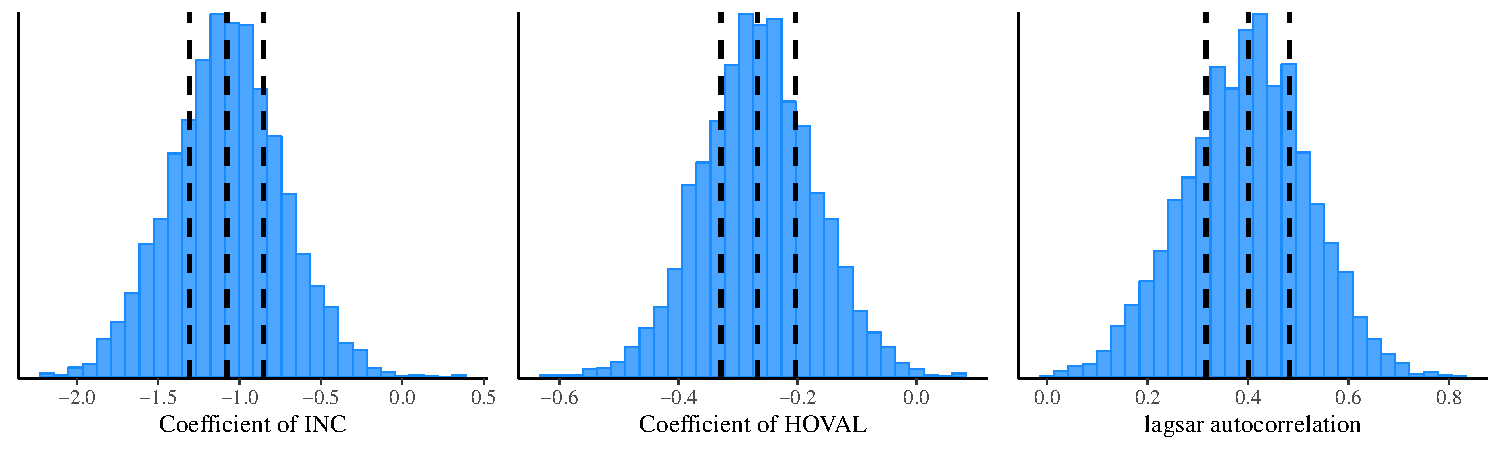
\includegraphics[width=0.95\linewidth]{plot-lagsar-1.pdf}
\caption{Posterior distribution of selected
parameters of the lagged SAR model along with posterior median and 50\%
central interval.}
\label{fig:plot-lagsar}
\end{figure}


After fitting the model, the next step is to compute the pointwise
log-likelihood values needed for approximate LOO-CV. To do this we use
the recipe laid out in Section \ref{sec-pointwise}. The quality of the PSIS-LOO
approximation can be investigated graphically by plotting the Pareto-\(k\) 
estimate for each observation. Ideally, they should not exceed \(0.5\), but 
in practice the algorithm turns out to be robust up to values of \(0.7\) 
\citep{vehtari2017loo,vehtari2017psis}. In Figure \ref{fig:psis-res-nb}, 
we see that the fourth observation is problematic and so may reduce the 
accuracy of the LOO-CV approximation.

\begin{figure}
\centering
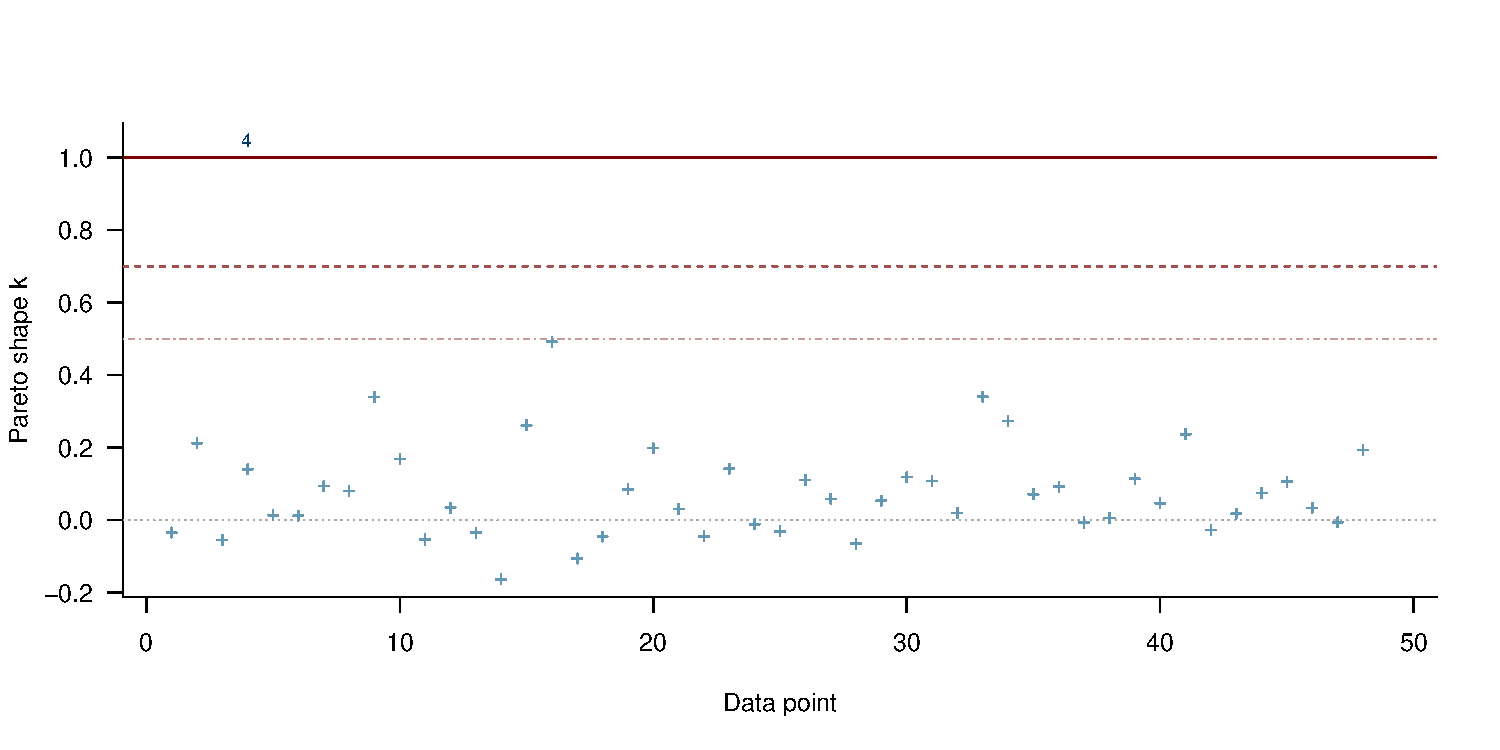
\includegraphics[width=0.95\linewidth]{psis-res-nb-1.pdf}
\caption{PSIS diagnostic plot showing the
Pareto-\(k\)-estimate of each observation.}
\label{fig:psis-res-nb}
\end{figure}

The PSIS-LOO-CV to approximation of the expected log predictive density
for new data reveals \(\text{elpd}_{\text{approx}} =\) -187.3. This
result still needs to be validated against exact LOO-CV, which is
somewhat more involved, as we need to re-fit the model \(N\) times each
time leaving out a single observations. For the lagged SAR model, we
cannot just ignore the held-out observation entirely as this will change
the prior of the other observations. In other words, the lagged SAR
model does not have the marginalization property that holds, for
instance, for Gaussian process models. Instead, we have to model the
held-out observation as a missing value, which is to be estimated along
with the other model parameters (see Section \ref{exact-loo}).

A first step in the validation of the pointwise predictive density is to
compare the distribution of the implied response values for the left-out
observation using the pointwise mean and standard deviation from
(\ref{ypredpars}) to the distribution of the \(y_i^{\mathrm{mis}}\)
posterior-predictive values estimated as part of the model. If the
pointwise predictive density is correct, the two distributions should
match very closely (up to sampling error). In Figure \ref{fig:yplots},
we overlay these two distributions for the first four observations and
see that they match very closely (as is the case for all
observations in this example).

\begin{figure}
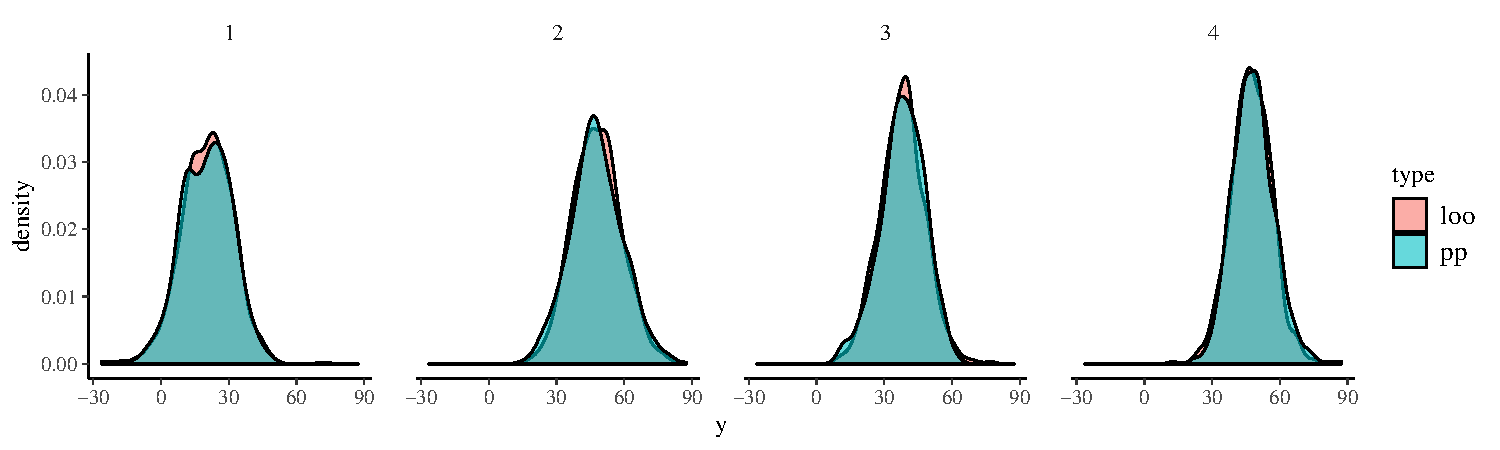
\includegraphics[width=0.95\linewidth]{yplots-1}
\caption{
Implied response values of the first four observations computed 
(a) after model fitting (type = 'loo') and 
(b) as part of the model in the form of posterior-predictive draws for the missing observation (type = 'pp').
}
\label{fig:yplots}
\end{figure}

In the final step, we compute the pointwise predictive density based on
the exact LOO-CV and compare it to the approximate PSIS-LOO-CV result
computed earlier. The results of the approximate
(\(\text{elpd}_{\text{approx}} =\) -187.3) and exact LOO-CV
(\(\text{elpd}_{\text{exact}} =\) -188.6) are similar but not as close
as we would expect if there were no problematic observations. We can
investigate this issue more closely by plotting the approximate against
the exact pointwise ELPD values.

\begin{figure}
\centering
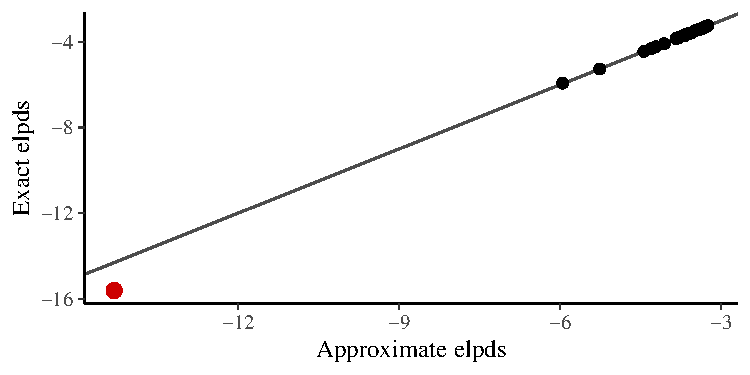
\includegraphics{elpd-compare-1.pdf}
\caption{Comparison of approximate and exact
pointwise elpd values for the SAR model. Problematic observations are
marked as red dots.}
\label{fig:elpd-compare}
\end{figure}

In Figure \ref{fig:elpd-compare}, the fourth data point -- the
observation flagged as problematic by the PSIS-LOO approximation -- is
colored in red and is the clear outlier. Otherwise, the correspondence
between the exact and approximate values is strong. In fact, summing
over the pointwise ELPD values and leaving out the fourth observation
yields practically equivalent results for approximate and exact LOO-CV
(\(\text{elpd}_{\text{approx},-4} =\) -172.9 vs.
\(\text{elpd}_{\text{exact},-4} =\) -173.0). From this we can conclude
that the difference we found when including \emph{all} observations does
not indicate an error in the implementation of the approximate LOO-CV
but rather a violation of its assumptions.


\section{Conclusion}

We have provided equations that enable both approximate and exact LOO-CV for
non-factorizable multivariate normal Bayesian models. Although exact LOO-CV is
usually impractical, our exact LOO-CV procedure can be used to validate the more
efficient PSIS-LOO-CV approximation.

The primary motivation for this paper is to enable approximate LOO-CV for models
that cannot be factorized at all, but our approach also works for \emph{any}
Bayesian model that can be expressed in terms of a multivariate normal
likelihood. Therefore it may also be useful for models that are factorizable but
for which the factorized representation is difficult to compute or not available
to the researcher for some other reason.


\bibliography{psis_non_factorizable}
\bibliographystyle{chicago}


%%: appendix
%\clearpage
%\section*{Appendix}

\end{document}
